\documentclass[11.5pt]{sig-alternate} % sets document style to sig-alternate
% packages
% typesetting
%\usepackage{dirtytalk} % typset quotations easier (\say{stuff})
\usepackage{hanging} % hanging paragraphs
\usepackage[defaultlines=3,all]{nowidow} % avoid widows
\usepackage[pdfpagelabels=false]{hyperref} % produce hypertext links, includes backref and nameref
\usepackage{xurl} % defines url linebreaks, loads url package
\usepackage{microtype}
\usepackage{textgreek}
%\usepackage{textcomp}
%\newcommand{\texttildemid}{\raisebox{0.4ex}{\texttildelow}}
% layout
\usepackage{enumitem} % control layout of itemize, enumerate, description
\usepackage{fancyhdr} % control page headers and footers
\usepackage{float} % improved interface for floating objects
%\usepackage{multicol} % intermix single and multiple column pages
% language
\usepackage[utf8]{inputenc} % accept different input encodings
\usepackage[english]{babel} % multilanguage support
% misc
\usepackage{graphicx} % builds upon graphics package, \includegraphics
%\usepackage{lastpage} % reference number of pages
%\usepackage{comment} % exclude portions of text (?)
\usepackage{xcolor} % color extensions
\usepackage[backend=biber, style=apa]{biblatex} % sophisticated bibliographies % necessary for HTML to display author info and date on abstract page
\usepackage{csquotes} % advanced quotations, makes biblatex happy
\usepackage{authblk} % support for footnote style author/affiliation
% tables and figures
\usepackage{tabularray}
%\usepackage{array} % extend array and tabular environments
\usepackage{caption} % customize captions in figures and tables (rotating captions, sideways captions, etc)
%\usepackage{cuted} % allow mixing of \onecolumn and \twocolumn on same page
\usepackage{multirow} % create tabular cells spanning multiple rows
%\usepackage{subfigure} % deprecated, support for manipulation of small figures
%\usepackage{tabularx} % extension of tabular with column designator "x", creates paragraph-like column whose width automatically expands
%\usepackage{wrapfig} % allows figures or tables to have text wrapped around them
%\usepackage{booktabs} % better rules
% dummy text
%\usepackage{blindtext} % blind text dummy text
%\usepackage{kantlipsum} % Kant style dummy text
\usepackage{lipsum} %lorem ipsum dummy text
% other helpful packages may be booktabs, longtable, longtabu, microtype

\pagestyle{fancy} % sets pagestyle to fancy for fancy headers and footers

% header and footer
% modern way to set header image
\renewcommand{\headrulewidth}{0pt} % defines thickness of line under header
\renewcommand{\footrulewidth}{0pt} % defines thickness of line above header
\setlength\headheight{80.0pt} % sets height between top margin and header image, effectively moves page contents down
\addtolength{\textheight}{-80.0pt} % seems to affect the lower height. maybe only works properly if footer numbers enabled?
\fancyhf{}
\fancyhead[CE, CO]{
\includegraphics[width=\textwidth]{headerImage.png}}
% footer
%\fancyfoot[LE,LO]{Article Title Here \\ DOI: }% left footer article title and doi
%\fancyfoot[CE,CO]{{}} % center footer empty
%\fancyfoot[RE,RO]{\thepage} % right footer page numbers
%\pagenumbering{arabic} % arabic (1, 2, 3) numbering in footer

\hypersetup{colorlinks=true,urlcolor=blue} % sets link color to blue
\urlstyle{same} % sets url typeface to same as rest of text

% set caption and figure to italics, label bold, left align captions, does not transfer to HTML
\captionsetup{labelfont=bf, font={large, it}, justification=raggedright, singlelinecheck=false}
\renewcommand\theContinuedFloat{\alph{ContinuedFloat}}

%this next bit is confusing, but essentially changes the width of the abstract. Seems to have been copied from this https://tex.stackexchange.com/questions/151583/how-to-adjust-the-width-of-abstract
\let\oldabstract\abstract
\let\oldendabstract\endabstract
\makeatletter %changes @ catcode to enable modification (in parsep)
\renewenvironment{abstract} %alters the abstract environment
{\renewenvironment{quotation}%
               {\list{}{\addtolength{\leftmargin}{1em} % change this value to add or remove length to the the default ?
                        \listparindent 1.5em%
                        \itemindent    \listparindent%
                        \rightmargin   \leftmargin%
                        \parsep        \z@ \@plus\p@}%
                \item\relax}%
               {\endlist}%
\oldabstract}
{\oldendabstract}
\makeatother %changes @ catcode to disable modification

% checks
% italics-
% links-
% dashes-
% tildes-
\begin{document}

\title{Students with Blindness Explore Chemistry at ‘Camp Can Do’}

\author[1]{\large \color{blue} Cary A. Supalo}
\author[2]{\large \color{blue} H. David Wohlers}
\author[3]{\large \color{blue} Jennifer R. Humphrey}


\affil[1]{Purdue University}
\affil[2]{Truman State University}
\affil[3]{Pennsylvania State University}
\toappear{}

\maketitle
\begin{@twocolumnfalse} 
\begin{abstract}
\item 
\begin{large}
\textit{Students with blindness or low vision are often discouraged from full participation in laboratory science classes due to the inadequacy of current methodological approaches and the lack of sophisticated adaptive technologies. Consequently, these students rarely go on to pursue advanced studies and employment in the sciences. In response to his own frustrations as a scientist with blindness, Supalo conceived, co-founded, and managed the Independent Laboratory Access for the Blind (ILAB) project for his doctoral research in chemistry. Numerous multisensory tools, technologies, and methodologies for teaching the sciences to students with visual impairments were developed and evaluated by the ILAB team. In 2009 and 2010, these hands-on adaptations were used by students with blindness and low vision from throughout the Caribbean during a chemistry workshop at a one-week summer camp held on the island of Tobago. Led by Supalo during the first-ever Camp Can Do in 2009 and Wohlers during 2010, the chemistry workshop successfully introduced the students to some basic chemical reactions and the most current adaptive technologies available for the laboratory sciences. For many of the students, Camp Can Do represented the first real opportunity to learn about science and technology with a hands-on approach.}
\\ \\
\end{large}     
\end{abstract}
\end{@twocolumnfalse}

%% ABSTRACT

%% AUTHOR INFORMATION

\textbf{*Corresponding Author, Cary A. Supalo}\\
\href{mailto:csupalo@purdue.edu}{(csupalo@purdue.edu)}\\
\textit{Submitted December 17, 2013}\\
\textit{Accepted December 17, 2013}\\
\textit{Published Online December 17, 2013}\\
\textit{DOI: 10.14448/jsesd.04.0001}\\

\pagebreak
\clearpage

\section*{INTRODUCTION}
\begin{large}
Traditionally, students who are blind or low vision (BLV) working in science laboratory classrooms have used what is referred to as the “directed laboratory assistant” approach, which consists of working with a sighted partner whom the BLV student instructs in carrying out the tasks of the laboratory activity (Miner, Nieman, Swanson, \& Woods, 2001, p. 62). While this approach has value — it’s effective in allowing students with BLV to complete course and degree requirements, and all current chemists with BLV have used it successfully to get where they are — it offers vicarious experiences that are not thoroughly motivating or engaging to a majority of participants. Supalo and Wohlers have observed firsthand that this lack of encouragement to explore science up close and personal, and the resulting lack of satisfaction, often deters students who are less than enthusiastic about science from pursuing further scientific efforts. This observation is supported by the fact that very few persons with disabilities, and even fewer with visual impairments in particular, are employed in chemistry or other scientific fields.

Information from the National Science Foundation (2006) revealed that only 6.5\% of the nation’s science and engineering professionals have disabilities. In 2009, an employment survey distributed to members of the American Chemical Society found that 2.2\% of respondents identified themselves as disabled (Allum, 2010). Of the persons with disabilities who were working in chemistry and named in the \textit{Resource Directory of Scientists and Engineers with Disabilities} (Stern, Mohamed, Summers, \& Leon, 2009), only a handful were visually impaired.

As scientists and educators who are blind, Supalo and Wohlers have always had a passion for working with persons with BLV, especially mentoring these individuals in science, technology, engineering, and mathematics (STEM). They believe that students with visual impairments can take fully active roles in science education and the science professions when provided with the appropriate adaptive tools.

While researching a problem in catalysis for his master’s thesis, Supalo encountered serious inconsistencies in results due to needing multiple undergraduates to assist him in the laboratory, who acted as his eyes and hands in handling the equipment and chemicals and performing tasks as directed. Due to the sensitivity of the reactions, any minor variations in technique from person to person introduced new, unwanted variables. As a result of these difficulties, for his Ph.D. research Supalo developed an interest in finding ways to allow persons with BLV to perform laboratory research in a more independent, hands-on manner. With the support of funding from the National Science Foundation’s Research in Disabilities Education program, he conceived, co-founded, and managed the Independent Laboratory Access for the Blind (ILAB) project at The Pennsylvania State University, which researched, developed, and evaluated multisensory tools, technologies, and methodologies for putting science literally within the grasp of high-school students with BLV (Supalo, 2007; Supalo, 2010; Supalo et al., 2006; Supalo et al., 2009; Supalo et al., 2007). These adaptations were field-tested in numerous mainstream high schools as well as residential schools for the blind.

In July 2009 Supalo brought some of the ILAB tools and technologies to the first-ever Camp Can Do, a one-week summer camp for youth with BLV on the Caribbean island of Tobago. This event, sponsored by The Torres Foundation for the Blind, included adaptive technology training workshops and experiential science activities, offering the opportunity to these students, many for the first time, to learn about science and technology with a hands-on approach, as well as participate in outdoor recreation, learn about self advocacy, and develop self confidence. Among the activities was a chemistry workshop headed by Supalo to introduce the students to various assistive tools to help them succeed in laboratory science. The 14 participants, most of whom were high-school age, along with a few a little younger or older, came from throughout the Caribbean, including Trinidad and Tobago, Jamaica, Barbados, and Antigua. The following summer, Wohlers taught the chemistry workshop at Camp Can Do 2010, featuring numerous all-new ILAB-adapted laboratory activities. Sixteen participants attended.

\section*{MAKING SCIENCE ACCESSIBLE}
The camp’s emphasis was on teaching the participants how to accomplish numerous STEM-related projects for themselves using a range of assistive hardware and software, not just that from ILAB. Among the technologies covered during various camp sessions were the Job Access with Speech (JAWS) text-to-speech screen reader, optical character recognition (OCR) software, and refreshable Braille display devices, all of which are widely possessed in the United States by people with BLV. Tools and techniques for measuring mass, volume, and length were also explored.

Available from Freedom Scientific, JAWS is a computer program for word processing and accessing online resources. It reads the text displayed on computer screens via synthesized speech, allowing persons with BLV to read and write reports, conduct online research, and otherwise access and manipulate computerized information. OCR software converts digitally scanned printed text into word-processing files and synthesized speech. Refreshable Braille display devices are likewise for reading from computer screens, through translating lines of text into Braille characters by means of raised pins, and can operate in conjunction with text-to-speech screen readers such as JAWS.

The ILAB tools used at Camp Can Do included an innovative interface between the JAWS screen reader and the standard Vernier laboratory hardware/software commonly found in science classrooms. The interface connects Vernier’s LabPro data-collection device, laboratory probes, and Logger Pro data-acquisition software to a PC via a standard USB cable, and thus to the JAWS program through specially developed JAWS scripting files (Supalo, 2010; Supalo et al., 2007). The interface can also be used with Vernier’s Go!Link devices instead of LabPro units, as was done at Camp Can Do 2010, when Wohlers used Go!Links rather than LabPros because the Go!Links were lighter and less expensive. Go!Links utilize Logger Lite data-acquisition software and accommodate only one probe at a time.

The JAWS interface allows extensive audible functionality with data collection, real-time probe readings, data table navigation, and statistical analysis. In short, with this setup, students with visual impairments can independently connect and install any desired sensors or probes, initiate data collection, and access and manipulate the resulting data.\textit{(Note: While laboratory probes are manufactured by multiple companies, the JAWS interface is usable only with Vernier products, which are widely available and inexpensive. Users may download the current JAWS scripting files needed to make JAWS compatible with Logger Pro from the ILAB Web site for free. Go to \url{http://ilab.psu.edu} and follow the directions.)}

\begin{figure}[htp]
    \centering
    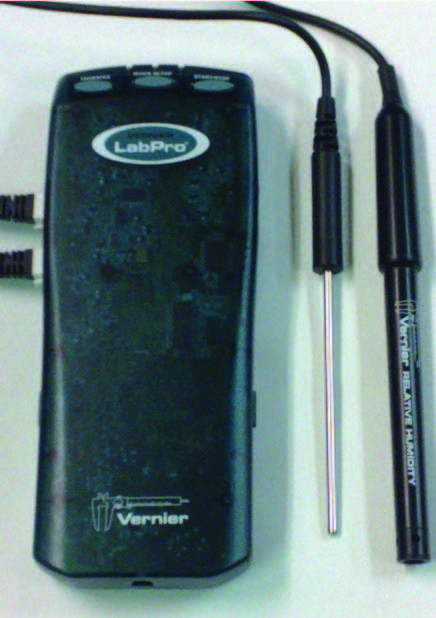
\includegraphics[width=\columnwidth]{Figure 1.jpg}
    \caption{Vernier LabPro with probes}
    \label{Figure 1}
\end{figure}

Another ILAB tool presented at Camp Can Do was a prototype device known as the Submersible Audible Light Sensor (SALS), developed in the Research Instruments Facility of the Chemistry Department at Penn State University (Supalo et al., 2006). The SALS, which incorporates a light sensor embedded in a glass wand, can measure color-intensity changes in a solution and convert the readings in real time to audible tones and synthesized speech indicating the hertz of the tone frequency. The tones produced by the SALS vary based on the amount of light detected. As a chemical reaction runs to completion, the intensity of light transmitted through the solution is modified as a result of the formation of a precipitate, a color change, or gas bubbles. The SALS also has memory storage capabilities so that tones can be played back for comparison purposes. Results can be qualitatively affected by shadows, such as those cast by students leaning over the equipment, but this is easily addressed.

\begin{figure}[htp]
    \centering
    \captionsetup{font=large, labelfont=it}
    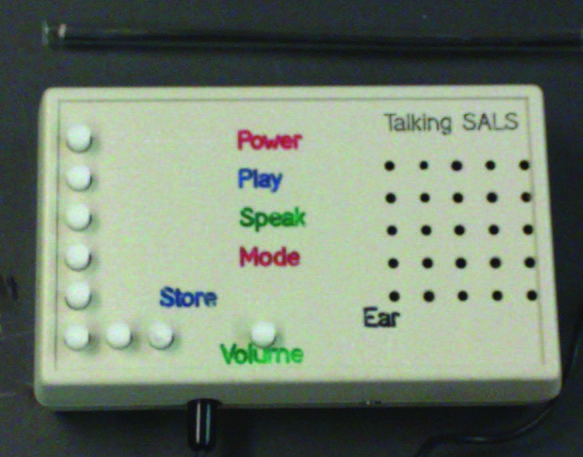
\includegraphics[width=\columnwidth]{Figure 2.jpg}
 \caption{\textit{The Submersible Audible Light Sensor (SALS) control box and probe}}
    \label{Figure 2}
\end{figure}

\subsection*{More About the SALS}
The Submersible Audible Light Sensor (SALS), developed by the Independent Laboratory Access for the Blind (ILAB) at Penn State University, may become commercially available within a couple of years. Meantime, the devices can be borrowed on a very limited basis from Cary Supalo by special request. Until the SALS is widely available for purchase by schools and teachers, there are some alternatives that can be adapted for laboratory classroom use.

One example is the telephone light sensor from Captek Inc., formerly Science Products for the Blind. The device was designed to detect the lights on telephones with multiple lines. While it is not submersible in liquids, it can detect color changes through glass, such as the walls of beakers or flasks. Before beginning development of the SALS, Supalo tested this limited application of the telephone light sensor and found it to be reasonably adequate, which fueled his interest in converting changes in light intensity to audible tones for laboratory classroom use by students with blindness or low vision.

The authors know of no submersible audible light sensors currently on the market from any manufacturer. Submersibility allows more effective measuring of even slight changes in light intensity in liquids, such as small variations in color or the formation of precipitates or bubbles, which the Captek product is not sensitive enough to detect. The SALS can also be used for separating clear liquids layered in the same vessel with a high degree of accuracy, detecting color changes of solid objects, and acid/base equivalency detection with the use of phenolphthalein (which is pink or red in basic solutions).

\section*{GETTING STUDENTS’ HANDS ONTO THE SCIENCE}
The 2009 chemistry workshop, held on the first day of camp, began with a discussion about the scientific method and how it can be used to problem solve. Next was a detailed demonstration of the ILAB tools and technologies. The Vernier probes were passed around for the participants to examine. The JAWS interface was then utilized with the probes and LabPro units to collect data on the temperature and humidity in the room. Data-table navigation was demonstrated by using the control-tab command and the corresponding up, down, left, and right arrow keys to read the individual data points in the table. A question-and-answer session regarding the functionality of these tools followed.

Various hands-on lab activities specifically adapt\-ed for persons with BLV were then conducted, including:

\textit{\textbf{What Happens When Alka Seltzer Meets Water?} The first hands-on activity consisted of each student placing an Alka Seltzer tablet into a zip-top plastic bag with 100 mL water, then listening to the results and tactilely exploring the formation of carbon dioxide gas from the reaction between the sodium bicarbonate, citric acid, and water (Chen \& Yaung, 2002; Huseth, 1998). The students could hear the bubbling of the gas being formed and feel the gas collecting in the plastic bag. This activity audibly and tactilely illustrated the three phases of matter — solid, liquid, and gas — and how matter can transform from one phase to the next.}

\textit{\textbf{Listening to the Iodine Clock Reaction.} In this activity, sodium thiosulfate, potassium iodide, sugar water, and ammonium peroxydisulfate were mixed together, and students working in small groups used the SALS to detect the reaction’s color changes over several minutes via modulations in the device’s audible tones. All initial solutions were pre-mixed and pre-measured into vials by the instructor, labeled on the lids using raised dots of glue, and provided to students by camp counselors. The reaction involved 10 mL of 0.0050M sodium thiosulfate solution and four drops of sugar water being added to 20 mL of 0.20M potassium iodide solution, then mixing the result with 20 mL of 0.10M ammonium peroxydisulfate (Wilbraham, Staley, \& Matta, 2002, pp. 235-241). A pie tin for use as a spill tray was distributed along with each SALS sensor. A Styrofoam cup was used as the reaction vessel. After the students mixed the solutions together, each student immediately inserted a SALS sensor into the reaction vessel to measure the initial tone, and stored this data in the device’s memory. With each sensor in the solution during the following five minutes, the tones decreased in pitch as the color of the solution evolved from clear to blue to brownish-black. When the tone began to change (within two or three minutes into the reaction), a second reading was stored. After the full five minutes of the reaction, a final reading was taken. The students compared the three tones, and the results were shared by each group with the entire class. Most of the students successfully recorded three different tones, audibly indicating the series of color changes. Thus, the SALS allowed the students to observe this chemical reaction through sound.}

The hands-on activities were followed by a second discussion about the scientific method and how it can be used to further describe various phenomena. Also discussed was how the evolution of a gas in the first activity indicated that a chemical reaction had occurred, and how the color changes in the second activity likewise indicated a reaction. The importance of knowing when a chemical reaction had occurred and how this differed from a simple physical change in matter was also covered.

The chemistry workshop at Camp Can Do 2010 featured a new set of laboratory activities, including:

\textit{\textbf{Cooling, Freezing, and Melting of Water.} After learning how to connect the temperature probe and familiarizing themselves with the appropriate keystrokes to hear the sensor readings, the campers added ice to warm water in a beaker and monitored the temperature drop by listening to the readings while the software collected the time-and-temperature data. Once the water-ice equilibrium temperature was reached at nearly 0 degrees Celsius, table salt was added. With gentle stirring, the students observed a further drop in temperature. This observation stimulated much enthusiasm. Each group tried to get to the lowest temperature possible. It was explained that the dissolved salt allowed the water-ice equilibrium temperature to lower, and that this would cause the freezing of water in a test tube to be placed in the beaker during the second part of the experiment. However, with only one temperature probe available per each of the four lab groups, it was important to demonstrate the temperature of the ice/water/salt mixture before conducting the freezing point determination. For the second part of the experiment, the students put the probe in a test tube filled with a small amount of water (about 5 mL), and the test tube was placed into the beaker containing the salt water. The students observed the phase change of the water inside the test tube from liquid to solid, then from solid back to liquid after the test tube was removed from the saltwater bath, while tracking the temperature throughout the entire process. Each team then examined the data table generated by the collection software through using the JAWS keystrokes to provide access.}

All scientific activities were preceded by a talk on safety in the laboratory. The importance of wearing safety goggles when doing experiments was discussed, and goggles were provided to all the students. This issue is as pertinent to students with visual impairments as it is to sighted students because chemical splashes in the eyes can still cause pain, impair any residual vision, and potentially damage prosthetic eyes. Proper dress was discussed, including wearing long pants and appropriate shoes. Additionally, emergency exit procedures were explained.

\section*{PROBLEM SOLVING FOSTERS INDEPENDENCE}
Through introduction to ILAB’s innovative technological and pedagogical research and development, the youth of the Caribbean with BLV have been exposed to the most current access technologies available for the laboratory sciences. The participants attended these camps with the expectation of learning more about themselves and how they could use access technologies to more fully engage with the world around them. The multisensory learning activities were designed as a series of confidence-building experiences to hopefully empower these students to seek more opportunities to participate both in STEM classes and in society in general, toward the goal of full inclusion in education, employment, and civic involvement.

The participants were asked how using the scientific method in everyday life could help persons with visual impairments become more independent. The group determined that their new observational skills, along with having access to assistive technologies, could allow persons with BLV to problem solve through various scenarios. In the end, all participants stated that they were able to relate the chemistry workshop experiences to aspects of their everyday lives at home and in school. They indicated they had come to understand that learning effective problem-solving skills and how to accurately observe phenomena in the laboratory were conducive to their personal independence as well as to their academic success.

Persons with BLV must use alternative means to collect information about their environment for everyday tasks such as getting from point A to point B independently, accessing the printed word, counting money, cooking, and innumerable other daily challenges. In fact, all persons with disabilities, not just those with blindness, must learn to become proficient in problem solving past their physical limitations. Doing so is essential to developing independence. The scientific method is a form of problem solving, and exploring scientific questions is valuable practice. It is the authors’ belief that the skills learned by young students in the laboratory during such practice can be transferred to their everyday lives.

\subsection*{Science Camps for Kids with Blindness or Low Vision}
Several other educational science camps exist in North America for students with visual impairments. Among them are:
\begin{itemize}
    \item Science Academy and Junior Science Academy, offered by the National Federation of the Blind (\url{www.blindscience.org/ncbys/Science_Academy.asp})
    \item Youth Slam*, offered in odd-numbered years by the National Federation of the Blind, for high school students (\url{www.blindscience.org/ncbys/Youth_Slam_20111.asp})
    \item Space Camp for Interested Visually Impaired Students, offered by the Texas School for the Blind and Visually Impaired, with separate programs for children in grades 4-6, 7-12, and 10-12. Held in Huntsville, Alabama, and open to participants from across the U.S. (\url{www.tsbvi.edu/space})
\end{itemize}
\textit{*Supalo has served as chemistry curriculum coordinator and/or instructor for Youth Slam since 2007 (Supalo et al., 2009).}

\section*{ACKNOWLEDGEMENTS}
Travel support for Supalo and Wohlers was provided by The Torres Foundation for the Blind. Further information on Camp Can Do and The Torres Foundation for the Blind can be found at \url{http://www.torresfoundation.org}. The National Science Foundation’s Research in Disabilities Education program supported the development and field testing of the ILAB tools used at this event (grants \#HRD-0726417 and \#HRD-0435656). Additionally, thanks go to the major members of the ILAB team, including Thomas Mallouk, George Bodner, Andrew Greenberg, April Hill, Rodney Kreuter, Alan Roth, Lillian Rankel, and Marilyn Winograd, who worked on the ILAB project along with Supalo and Wohlers. Thanks also go to all teachers and students who participated in the research and field testing of the ILAB tools throughout the course of the project. More about the ILAB project can be found at \url{http://ilab.psu.edu}.

\section*{BIOGRAPHICAL STATEMENTS}
\textbf{Cary Supalo} \href{mailto:csupalo@purdue.edu}{(csupalo@purdue.edu)}, who lost his sight in early childhood, is currently a visiting scientist in chemical education at Purdue University. He completed his Ph.D. in chemistry, with an emphasis in chemical education, in fall 2010 at The Pennsylvania State University. He co-founded ILAB in 2004 and managed the project for the six years of its active existence. For his dissertation, he field tested the ILAB tools in 12 mainstream high schools across the U.S. and is currently completing analyses of the data. In 2009 he founded and is president of Independence Science LLC, a business offering consulting services and assistive hardware/software to school districts, state rehabilitation agencies, colleges and universities, and students and parents. In helping students with blindness or low vision to have hands-on science learning experiences, Independence Science is continuing the work begun during the ILAB project.

\textbf{H. David Wohlers} \href{mailto:wohlers@truman.edu}{(wohlers@truman.edu)}, who likewise has been blind since early childhood, is a professor of chemistry at Truman State University and was twice elected as chair of the Chemistry Department. He has taught undergraduate chemistry since receiving his Ph.D. in 1983. Among the professionals with visual impairments listed in the AAAS’s Resource Directory of Scientists and Engineers with Disabilities and a CareerConnect mentor with the American Foundation for the Blind, he has offered encouragement and advice both to colleagues encountering students with blindness and to college students with visual impairments taking science courses for the first time. Wohlers has been a mentor and friend to Supalo since 1996 and participated in the two NSF grants that supported the ILAB project.

\textbf{Jennifer R. Humphrey} \href{mailto:jrh49@psu.edu}{(jrh49@psu.edu)} is employed in the Chemistry Department and the Office for Disability Services at The Pennsylvania State University, and is also an independent writer, editor, and researcher. She has 20 years of experience as a writing/editing professional, and has worked closely with Supalo since 2008. She has degrees in earth science and English, and is sighted.

\clearpage
\end{large}
\section*{REFERENCES}\par 

\leftskip 0.25in
\parindent -0.25in 

Allum, J.R. (2010). \textit{Annual salary and employment survey 2009}. Washington, DC: American Chemical Society.

Chen, Y.-H., \& Yaung, J.-F. (2002). Alka Seltzer fizzing – Determination of percent by mass of NaHCO3 in Alka Seltzer tablets. \textit{Journal of Chemical Education}, 79, 848-850.

Huseth, A. (1998). The science mentor: An adventure in chemistry education. \textit{Journal of Chemical Education}, 75, 528A-528B.

Miner, D.L., Nieman, R., Swanson, A.B., \& Woods, M. (Eds.). (2001). \textit{Teaching chemistry to students with disabilities: A manual for high schools, colleges, and graduate programs} (4th ed.). Washington, DC: American Chemical Society.

National Science Foundation, Division of Science Resource Statistics, Scientists and Engineers Statistical Data System. (2006). \textit{Table 9-8: Employed scientists and engineers, by occupation, highest degree level, and disability status: 2006}. Arlington, VA: Author. Retrieved from \url{http://www.nsf.gov/statistics/wmpd/pdf/tab9-8.pdf}

Stern, V.W., Mohamed, S., Summers, L., \& Leon, T. (Eds.). (2009). \textit{Resource directory of scientists and engineers with disabilities} (4th ed.). Washington, DC: American Association for the Advancement of Science.

\newpage Supalo, C. (2007). Independent Laboratory Access for the Blind. \textit{Braille Monitor}, 50 (5). Retrieved from \url{http://www.nfb.org/Images/nfb/Publications/bm/bm07/bm0705/bm070506.htm}

Supalo, C.A. (2010). \textit{Teaching chemistry and other sciences to blind and low-vision students through hands-on learning experiences in high school science laboratories} (Doctoral dissertation). Available from ProQuest Dissertations and Theses database. (UMI 3442959)

Supalo, C., Kreuter, R.A., Musser, A., Han, J., Briody, E., McArtor, C., Gregory, K., \& Mallouk, T.E. (2006). Seeing chemistry through sound: A submersible audible light sensor for observing reactions in real time. \textit{Assistive Technology Outcomes and Benefits}, 3, 110-116.

Supalo, C.A., Mallouk, T.E., Amorosi, C., Lanouette, J., Wohlers, H.D., \& McEnnis, K. (2009). Using adaptive tools and techniques to teach a class of students who are blind or low-vision. \textit{Journal of Chemical Education}, 86, 587-591.

Supalo, C.A., Mallouk, T.E., Amorosi, C., Rankel, L.A., Wohlers, H.D., Roth, A., \& Greenberg, A. (2007). Talking tools to assist students who are blind in laboratory courses. \textit{Journal of Science Education for Students with Disabilities}, 12, 27-32.

Wilbraham, A.C., Staley, D.D., \& Matta, M.S. (2002). \textit{Chemistry laboratory manual: Teacher’s edition}. Upper Saddle River, NJ: Prentice-Hall.

\end{document}
